\section{数学模型}

\subsection{拉普拉斯变换}

定义:

\begin{align*}
f(t)&=\mbox{时间$t$的函数,并且当$t<0$时$f(t)=0$}\\
s&=\mbox{复变量}\\
\Laplace&=\mbox{运算符号,表示该量用拉普拉斯积分$\int_0^\infty e^{-st}dt$进行变换}\\
F(s)&=f(t)\mbox{的拉普拉斯变换}
\end{align*}

于是,$f(t)$的拉普拉斯变换为

\begin{equation*}
\Laplace[f(t)]=F(s)=\int_0^\infty e^{-st}dt[f(t)]=\infty_0^\infty f(t)e^{-st}dt
\end{equation*}

从拉普拉斯变换$F(s)$求时间函数$f(t)$的反变换过程称为拉普拉斯反变换:

\begin{equation*}
\Laplace^{-1}[F(s)]=f(t)=\frac{1}{2\pi j}\int_{c-j\infty}^{c+j\infty}F(s)e^{st}ds
\end{equation*}

一般不通过计算反演积分来求拉普拉斯反变换,多数情况可以通过部分分式展开再查表来求$f(t)$。

初值定理:

\begin{equation*}
f(0+)=\lim_{t\to0+}f(t)=\lim_{s\to\infty}sF(s)
\end{equation*}

终值定理:

\begin{equation*}
f(\infty)=\lim_{t\to \infty}f(t)=\lim_{s\to0}sF(s)
\end{equation*}

在复平面上,使复变函数$G(s)$解析(满足柯西-黎曼条件)的点称为普通点,使其非解析的点称为奇点;使$G(s)$或其导数趋近于无穷大的奇点称为极点,使$G(s)$等于零的奇点称为零点。

$s$趋近于$p$时,$G(s)$趋于无穷大,且$G(s)(s-p)^n$在$s=p$处取到一个非零的有限值,则称该极点为$n$阶极点。

\subsection{傅里叶变换}

用$j\omega$代替拉普拉斯变换中的$s$,即可得到傅里叶变换,其中的$\omega$为频率,其单位为$rad/s$;当使用频率单位为周/秒进行测量时,用$f$表示,$\omega=2\pi f$。

\begin{equation*}
F(j\omega)=\Fourier[f(t)]=\int_{-\infty}^\infty f(t)e^{-j\omega t}dt
\end{equation*}

对应的傅里叶逆变换:

\begin{equation*}
f(t)=\Fourier^{-1}[F(j\omega)]=\frac{1}{2\pi}\int_{-\infty}^\infty f(t)e^{j\omega t}d\omega
\end{equation*}



\subsection{传递函数}

对于微分方程

\begin{align*}
a_0y^{(n)}+a_1y^{(n-1)}&+\cdots+a_{n-1}\dot y+a_ny\\
&=b_0x^{(m)}+b_1x^{(m-1)}+\cdots+b_{m-1}\dot x+b_mx\hspace{2em}(n\ge m)
\end{align*}

式中,$x$为输入,$y$为输出,其对应的传递函数定义为输入与输出的拉普拉斯变换的比值:



\begin{equation*}
\begin{aligned}
\mbox{传递函数}&:=G(s)\\
&=\frac{\Laplace[\mbox{输出量}]}{\Laplace[\mbox{输入量}]}\Big|_{\mbox{零初始条件}}\\
&=\frac{Y(s)}{X(s)}\\
&=\frac{b_0s^m+b_1s^{m-1}+\cdots+b_{m-1}s+b_m}{a_0s^n+a_1s^{n-1}+\cdots+a_{n-1}+a_n}
\end{aligned}
\end{equation*}

传递函数中,如果分母$s$的最高阶次为$n$,则称系统为$n$阶系统。

\subsection{卷积积分}
由传递函数的定义,可以得到

\begin{equation*}
Y(s)=G(s)X(s)
\end{equation*}

由拉普拉斯变换的性质可知,复域内的乘法等价于时域内的卷积,因此有

\begin{align*}
y(t)&=\int_0^tx(\tau)g(t-\tau)d\tau\\
&=\int_0^tg(\tau)x(t-\tau)d\tau
\end{align*}

\subsection{脉冲响应函数}

同样地,由传递函数的定义可以知道,如果能找到一个输入函数,其拉普拉斯变换为$1$(准确来讲是单位阶跃函数$u(t)$),那么就能得到

\begin{equation*}
Y(s)=G(s)
\end{equation*}

此时需要的输入函数就应当是单位脉冲函数$\delta(t)$

\begin{equation*}
x(t)=\Laplace^{-1}[1]=\delta(t)
\end{equation*}

对输出量进行拉普拉斯反变换,得到的函数即称为脉冲响应函数,


\begin{equation*}
\Laplace^{-1}[G(s)]=g(t)
\end{equation*}

脉冲响应函数的意义是,当初始条件为$0$时,对系统输入一个单位脉冲函数,此时得到的输出。对这个脉冲响应函数作拉普拉斯变换,即可得到传递函数$G(s)$。

\subsection{闭环传递函数的等效}


\begin{figure}[!ht]
	\centering
	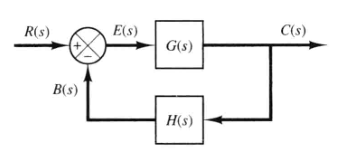
\includegraphics[width=8cm]{figures/2.png}
	\caption{闭环控制系统方块图}
	\label{2}
\end{figure}



如图\ref{2}所示的闭环控制系统,输出量$C(s)$与输入量$R(s)$之间的关系有
\begin{align*}
C(s)&=G(s)E(s)\\
E(s)&=R(s)-B(s)\\
&=R(s)-C(s)H(s)
\end{align*}

消去$E(s)$,从而有
\begin{align*}
C(s)&=G(s)[R(s)-H(s)C(s)]\\
[1+G(s)H(s)]C&=G(s)R(s)\\
\frac{C(s)}{R(s)}&=\frac{G(s)}{1+G(s)H(s)}
\end{align*}

这个式子可以消去反馈回路,化简方块图。

\subsection{非线性系统的线性化}

一个系统如果不能满足叠加原理,则该系统是非线性系统。但考虑到线性系统的优良性质,并且实际状况下,系统围绕着平衡点工作,将信号视为围绕平衡点变化的小信号,就可以用线性系统来近似非线性系统。对于非线性系统,输入为$u(t)$,输出为$y(t)$,满足关系

\begin{equation*}
	f(y^{(n)},y^{(n-1)},\cdots,y',y,u^{(m)},u^{(m-1)},\cdots,u',u)=0
\end{equation*}

线性化的具体的做法如下:

\begin{enumerate}
	\item 求平衡状态。令式中$u$和$y$的各阶导数均为0,结合给定的限制条件(对平衡位置的要求),得到平衡状态下的$\bar{u}$,$\bar{y}$:
	
	\begin{equation*}
		f(0,0,\cdots,0,\bar{y},0,0,\cdots,0,\bar{u})=0
	\end{equation*}

	\item 将原输入、输出$u$,$y$映射为新的变量$\delta_u$,$\delta_y$:
	
	\begin{align*}
		\delta_u&=u-\bar{u}\\
		\delta_y&=y-\bar{y}
	\end{align*}

	显然,对应的导数不发生变化:

	\begin{align*}
		\frac{d^k\delta_y}{dt^k}&=\frac{d^ky}{dt^k}\\
		\frac{d^k\delta_u}{dt^k}&=\frac{d^ku}{dt^k}
	\end{align*}

	\item 利用泰勒展开,只取第一项,得到对应的线性化系统(每项偏导均代入平衡状态下的取值)
	
	\begin{align*}
		&f(y^{(n)},y^{(n-1)},\cdots,y',y,u^{(m)},u^{(m-1)},\cdots,u',u)\\
		=&f(0,0,\cdots,0,\bar{y},0,0,\cdots,0,\bar{u})\\
		&\phantom{aaa}+\frac{\partial f}{\partial y^{(n)}}(y^{(n)}-0)+\frac{\partial f}{\partial y^{(n-1)}}(y^{(n-1)}-0)+\cdots+\frac{\partial f}{\partial y}(y-\bar{y})\\
		&\phantom{aaa}+\frac{\partial f}{\partial u^{(m)}}(u^{(m)}-0)+\frac{\partial f}{\partial u^{(m-1)}}(u^{(m-1)}-0)+\cdots+\frac{\partial f}{\partial u}(u-\bar{u})\\
		=&0+\frac{\partial f}{\partial y^{(n)}}\delta_y^{(n)}+\frac{\partial f}{\partial y^{(n-1)}}\delta_y^{(n-1)}+\cdots+\frac{\partial f}{\partial y}\delta_y\\
		&\phantom{aaa}+\frac{\partial f}{\partial u^{(m)}}\delta_u^{(m)}+\frac{\partial f}{\partial u^{(m-1)}}\delta_u^{(m-1)}+\cdots+\frac{\partial f}{\partial u}\delta_u\\
		=&f_{lin}(\delta_y^{(n)},\delta_y^{(n-1)},\cdots,\delta_y',\delta_y,\delta_u^{(m)},\delta_u^{(m-1)},\cdots,\delta_u',\delta_u)=0\\
	\end{align*}
\end{enumerate}




\subsection{用MATLAB求传递函数}

定义传递函数可以利用MATLAB中的\textit{tf}函数。例如,要定义传递函数

\begin{equation*}
	G(s)=\frac{s^2-2s+16}{3s+1}
\end{equation*}

可以这样来定义:

\begin{lstlisting}
s=tf('s');
sys{1}=(s^2-2*s+16)/(3*s+1)
\end{lstlisting}

此外,还可以通过函数\textit{step}和函数\textit{bode}来求取对应的阶跃响应和频响特性曲线。

\begin{figure}[!ht]
	\centering
	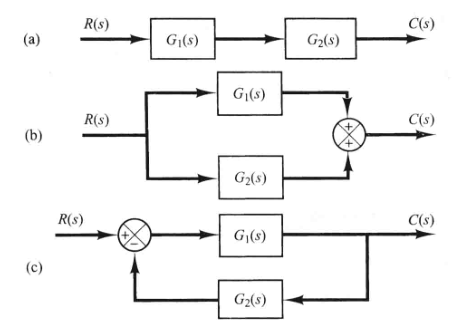
\includegraphics[width=8cm]{figures/1.png}
	\caption{串联、并联与闭环反馈}
	\label{1}
\end{figure}

对于串联、并联和闭环反馈形式的传递函数,如图\ref{1},可以用这样的MATLAB命令来定义:

\begin{lstlisting}
[num,den] = series(num1,den1,num2,den2)
[num,den] = parallel(num1,den1,num2,den2)
[num,den] = feedback(num1,den1,num2,den2)
\end{lstlisting}

比如,对于传递函数$G_1(s)$和$G_2(s)$的闭环反馈
\begin{equation*}
G_1(s)=\frac{10}{s^2+2s+10}=\frac{num1}{den1},\hspace{2em}G_2(s)=\frac{5}{s+5}=\frac{num2}{den2}
\end{equation*}

可以用下面的代码实现

\begin{lstlisting}
num1 = [10];
den1 = [1,2,10];
num2 = [5];
den2 = [1,5];
[num,den] = feedback(num1,den1,num2,den2);
printsys(num,den)
\end{lstlisting}